
\documentclass[tikz,border=2pt]{standalone}
\usepackage{tikz}
\usepackage{lmodern}
\usetikzlibrary{calc,decorations.pathreplacing}

% Visual conventions follow the existing MRNC TikZ pictures: ordinary
% components use TikZ's normal 0.4pt stroke, with compact TeX labels.
\tikzset{
  nu fibre/.style={
    x=0.78cm,
    y=0.78cm,
    line width=0.4pt,
    line cap=round,
    line join=round
  },
  nu label/.style={
    font=\scriptsize,
    inner sep=1pt
  },
  nu annotation/.style={
    font=\scriptsize,
    inner sep=1pt
  },
  nu dots/.style={
    font=\small,
    inner sep=0pt
  }
}

\begin{document}

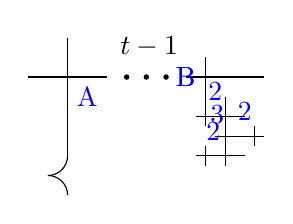
\begin{tikzpicture}[scale=0.5]
              %chain
  \coordinate (C) at (-1.50, 3.00);
  \coordinate (D) at (-0.50, 3.00);
  \coordinate (A) at (-1.00, 3.00);
  \coordinate (B) at (-0.93, 3.26);
\node[above] at (B) {$t-1$};
  \fill[black] (C) circle (2pt);
  \fill[black] (D) circle (2pt);
  \fill[black] (A) circle (2pt);
 
   %II 
    
   \coordinate (IIlP) at (-4.00, 3.00);
  \coordinate (IIlQ) at (-2.00, 3.00);
  \coordinate (IIlR) at (-3.00, 4.00);
  \coordinate (IIlS) at (-3.00, 1.00);
 \coordinate (IIlT) at (-3.50, 1.00);
  \coordinate (IIlU) at (-3.50, 0.00);
  \coordinate (IIlA) at (-2.50, 2.00);
  \draw (IIlP) -- (IIlQ);
  \draw (IIlR) -- (IIlS);
  \draw (-3.00, 1.00) arc (0.0:-90.0:0.50);
  \draw (-3.50, 0.50) arc (90.0:0.0:0.50);
  \node[above, text=blue] at (IIlA) {A};

%IV^*


  \coordinate (IVSSlA) at (0.00, 3.00);
  \coordinate (IVSSlB) at (2.00, 3.00);
  \coordinate (IVSSlC) at (0.50, 3.50);
  \coordinate (IVSSlD) at (0.50, 1.75);
  \coordinate (IVSSlE) at (0.25, 2.00);
  \coordinate (IVSSlF) at (1.50, 2.00);
  \coordinate (IVSSlG) at (1.00, 2.50);
  \coordinate (IVSSlH) at (1.00, 0.75);
  \coordinate (IVSSlI) at (0.75, 1.50);
  \coordinate (IVSSlJ) at (2.0, 1.50);
  \coordinate (IVSSlK) at (1.75, 1.75);
  \coordinate (IVSSlL) at (1.75, 1.25);
  \coordinate (IVSSlM) at (0.25, 1.00);
  \coordinate (IVSSlN) at (1.50, 1.00);
  \coordinate (IVSSlO) at (0.50, 1.25);
  \coordinate (IVSSlP) at (0.50, 0.75);
  \coordinate (IVSSlR) at (0.75, 2.16);
  \coordinate (IVSSlQ) at (0, 2.50);
  \coordinate (IVSSlS) at (1.5, 1.64);
  \coordinate (IVSSlU) at (0.8, 1.56);
  \coordinate (IVSSlV) at (0.7, 1.15);


  \draw (IVSSlA) -- (IVSSlB);
  \draw (IVSSlG) -- (IVSSlG);
  \draw (IVSSlG) -- (IVSSlG);
  \draw (IVSSlC) -- (IVSSlD);
  \draw (IVSSlE) -- (IVSSlF);
  \draw (IVSSlG) -- (IVSSlG);
  \draw (IVSSlG) -- (IVSSlH);
  \draw (IVSSlG) -- (IVSSlH);
  \draw (IVSSlI) -- (IVSSlI);
  \draw (IVSSlI) -- (IVSSlJ);
  \draw (IVSSlF) -- (IVSSlF);
  \draw (IVSSlF) -- (IVSSlF);
  \draw (IVSSlK) -- (IVSSlK);
  \draw (IVSSlJ) -- (IVSSlJ);
  \draw (IVSSlJ) -- (IVSSlJ);
  \draw (IVSSlF) -- (IVSSlF);
  \draw (IVSSlK) -- (IVSSlL);
  \draw (IVSSlK) -- (IVSSlL);
  \draw (IVSSlM) -- (IVSSlN);
  \draw (IVSSlI) -- (IVSSlI);
  \draw (IVSSlI) -- (IVSSlI);
  \draw (IVSSlO) -- (IVSSlP);
  \node[above, text=blue] at (IVSSlQ) {B};
  \node[above, text=blue] at (IVSSlR) {$2$};
  \node[above, text=blue] at (IVSSlQ) {B};
  \node[above, text=blue] at (IVSSlS) {$2$};

  \node[above, text=blue] at (IVSSlU) {$3$};
  \node[above, text=blue] at (IVSSlV) {$2$};

\end{tikzpicture}

\end{document}
